\section{Benchmark Datasets}
This section will outline some of the commonly used object detection datasets. This will include their purpose and the general setup.


\subsection{PASCAL Visual Object Classes Challenge}
The \gls{pascalvoc} challenge \cite{pascalvoc2012} was held yearly between 2005 to 2012 and provided datasets for benchmarking within vision tasks of visual object category recognition and detection. Between that time period is was considered the top benchmark for the respective challenges. While being an annual competition, \gls{pascalvoc} evaluation in state-of-the-art literature is most often performed on data from the years 2007 and 2012. The competition saw a large shift in the former year as the number of classes increased from 10 to 20, in turn also significantly increasing the total amount of data. Additional data was added individually for the various recognition tasks between 2007 and 2012 and the performance metric was altered slightly between this time period, however, the overall ecosystem remained largely the same from 2007 until the competition's end. This section will be largely based upon the two retrospective papers, \cite{pascalvoc2010} and \cite{pascalvoc2015}, published by authors who were involved in the challenge and for the most part will be in respect to the challenge after 2007.
\\\\
Images were obtained from the website flickr \cite{flickr} with the aim in mind to collect natural images for the recognition challenges. Ideally the dataset was to contain a significant level of visual variability in regards to object size, orientation, pose, illumination, position, and occlusion. A total of 20 classes were present in the 2007 challenges and these remained the same until 2012. The classes can be considered as a part of a taxonomy with 4 main branches, where each has finer-grain objects in sub-classes. The 20 classes and the branching taxonomy can be seen in \tableref{vocclasses}.


\begin{table}[h]
\centering
\caption{Taxonomy of the 20 classes introduced in VOC2007.}
\label{tab:vocclasses}
\begin{tabular}{llll}
\hline
Vehicles & Household & Animals & Other \\ \hline
Aeroplane                      & Bottle                         & Bird                         & Person                     \\
Bicycle                        & Chair                          & Cat                          &                            \\
Boat                           & Dining table                   & Cow                          &                            \\
Bus                            & Potted plant                   & Dog                          &                            \\
Car                            & Sofa                           & Horse                        &                            \\
Motorbike                      & TV/Monitor                     & Sheep                        &                            \\ \hline
Train    &  &  &  \\ \hline
\end{tabular}
\end{table}

A total of 500,000 potential images were collected randomly based upon different combinations of queries for a given class. For example of class bird, potential queries were bird, birdie, birdwatching, nest, sea, aviary, birdcage, bird feeder, and bird table. Of these potential images the majority were discarded for potential annotation due to not meeting the considerations of visual variability mentioned earlier. The annotation process was completed by a team from the University of Leeds based upon strict guidelines. The aim was to ensure that the annotations resulted in a consistent, accurate, and exhaustive dataset. The annotations are stored in XML format which contains the following information:

\begin{itemize}
	\item Class: one of the 20 shown in \tableref{vocclasses}.
	\item Bounding box: axis-aligned bounding-box around the visual extent of the object.
	\item Viewpoint: viewpoint to the object.
	\item Truncation: whether or not object is truncated. An object is truncated when the bounding-box does not cover the full extent of the object. Truncation can occur if the object extends outside the image or is partially occluded.
	\item Difficult: A subjective evaluation on if the object is difficult to detect. This is determined based on object size, illumination, or image quality.
\end{itemize}

An example of the XML format for the object chair can be seen in Code \ref{lst:xml_ex} and its corresponding image in \figref{xml_eximg}. 

\begin{lstlisting}[language=xml,caption={Example of XML annotation for the object chair.}
\label{lst:xml_ex}]
<object>
    <name>chair</name>
    <pose>Rear</pose>
    <truncated>0</truncated>
	<difficult>0</difficult>
	<bndbox>
		<xmin>263</xmin>
		<ymin>211</ymin>
		<xmax>324</xmax>
		<ymax>339</ymax>
	</bndbox>
</object>
\end{lstlisting}

\begin{figure}[H]
  \centering
    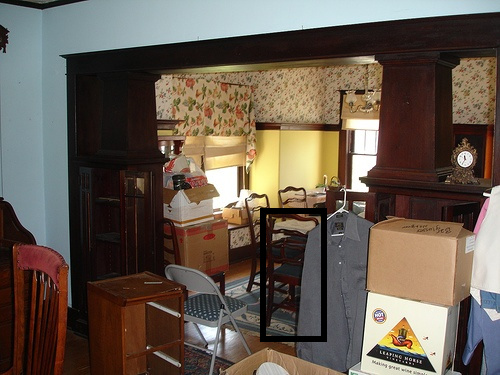
\includegraphics[width=0.7\textwidth]{Figs/Techanal/000005.jpg}
    \caption{Image from the \gls{pascalvoc} 2007 dataset. The bounding box represents the annotated XML data shown in Code \ref{lst:xml_ex}.}
    \label{fig:xml_eximg}
\end{figure}

Of the 500,000 potential images, 9,963 were annotated for the VOC2007 challenges based upon the annotation guidelines. \gls{pascalvoc} datasets is split into two subsets; \lstinline{trainval}, consisting of training and validation data and \lstinline{test}, consisting of the testing data. A histogram showing the frequency of an object class in an image and the total number of objects for the VOC2007 dataset can be seen in \figref{vochist07}.

\begin{figure}[H]
  \centering
    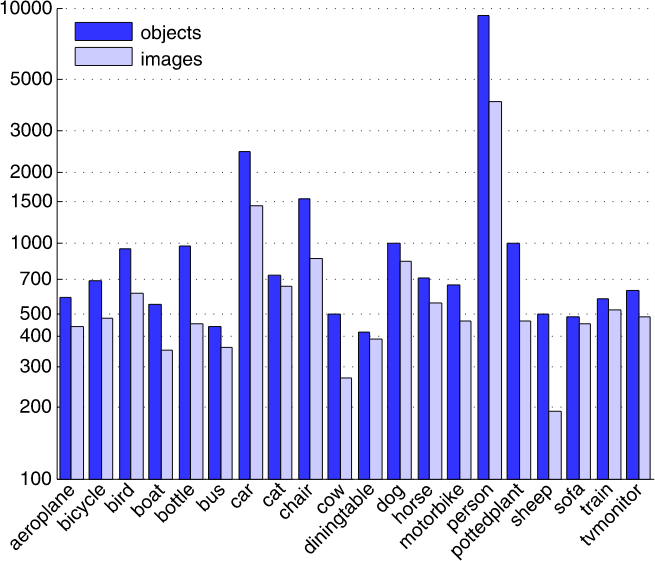
\includegraphics[width=0.5\textwidth]{Figs/Techanal/vochist07.png}
    \caption{Image from the \gls{pascalvoc} 2007 dataset. The bounding box represents the annotated XML data shown in Code \ref{lst:vochist07}.}
    \label{fig:vochist07}
\end{figure}


Evaluation of a object detector on \gls{pascalvoc} is based upon \gls{ap} which summarises the precision and recall of detections. The metric requires that for each detection both a bounding-box and an associated confidence. With these a precision/curve can be calculated and the overall \gls{ap} for the curve represents the performance of the detector. By altering the threshold corresponding to the confidence of each detection a precision and recall curve can be calculated and the \gls{ap} summarises the shape of the this. Precision is the number of true positives in relation to both true positives and false positives. Whereas, recall is the number of true positives in relation to all detections. However firstly, a detection must be classified as either a true or false positive. This is determined by measuring the bounding-box overlap between the detection and ground truth annotation. In \gls{pascalvoc} a bounding box is a true positive if the overlap is above 50\% according to the following calculation:

\begin{equation}\label{pascalBB}
	a_o = \frac{area(B_p \bigcap B_{gt})}{area(B_p \bigcup B_{gt})}
\end{equation}
 
where $B_p \bigcap B_{gt}$ is the intersection of the predicted bounding box and the ground truth and $B_p \bigcup G_{gt}$ is the union between the two. It should also be noted that for a given ground truth object it is only possible to have one true positive detection. If multiple detections satisfy Equation \ref{pascalBB} the remaining will be denoted as a false positive. Now that detections can be as classified as either a true or false positive \gls{ap} can be calculated. Before 2007, in \gls{pascalvoc} this was calculated as the mean precision at eleven equally space recalls [0, 0.1, ..., 1] by:

\begin{equation}
	AP = \frac{1}{11} \sum_{r\epsilon[0, 0.1, ..., 1]}p_{interp}(r)  
\end{equation}

where $r$ is the recall and $p_{interp}$ is the interpolated precision.
\add[inline]{explanation of interpolated precision}
\add[inline]{explanation of new metric}


\subsection{Microsoft Common Object in Context}
\gls{mscoco} \cite{mscoco} is a relatively new dataset within the realm of object recognition appearing in 2015. \gls{mscoco} holds competitions in object detection and segmentation. The object detection challenge is similar to \gls{pascalvoc}, in that detections must be shown using bounding-boxes. However, for the segmentation challenge \gls{mscoco} requires the results to be of more challenging instance form rather than semantic. The creators of the dataset had three core research problems they wanted to be present, these include:

\begin{enumerate}
	\item Detecting non-iconic views of objects.
	\item Contextual reasoning between objects.
	\item Precise 2-dimensional localisation of objects.
\end{enumerate}

The first problem is present by having object instances in images that are closer to everyday scenarios. Iconic views of objects are when the instance is near the centre of the image, is unobstructed and taken in a controlled scenario. Objects taken in such conditions are much easier to detect but practical applications are limited. Therefore, non-iconic views of objects are collected by having images that can have background or other objects present, objects being partially occluded and being amongst clutter. By having a dataset of non-iconic views, the second research problem is addressed as objects are in scenarios where context with respect to the scene can be used. Finally, a higher level of precision is provided in the \gls{mscoco} segmentation challenge. As mentioned, results are required to be instance and pixel-wise. Therefore, the objects in the dataset are annotated precisely at a pixel-level but also with coarser bounding-boxes. These goals resulted in a dataset has a total of 91 object classes of which 82 have more than 5,000 labelled instances. Considerably higher that that of \gls{pascalvoc}. In addition to having a large number of classes the number of object instance per image is also relatively high. On average there is 7.7 instances per image, considerably higher than \gls{pascalvoc} with 2.3 and ImageNet with 3.0. 
\\\\
The object classes chosen are similar to those in \gls{pascalvoc}, where the categories should represent a common objects that are relevant to practical applications. Also the categories should be such that a high number of images that respect the core research problems can be found. The 91 categories were chosen to be at a higher-level of taxonomy such that they would be the commonly used label by a typical person. The categories and number of instances in each can be seen in \figref{cocoinstances}.

\begin{figure}[H]
  \centering
    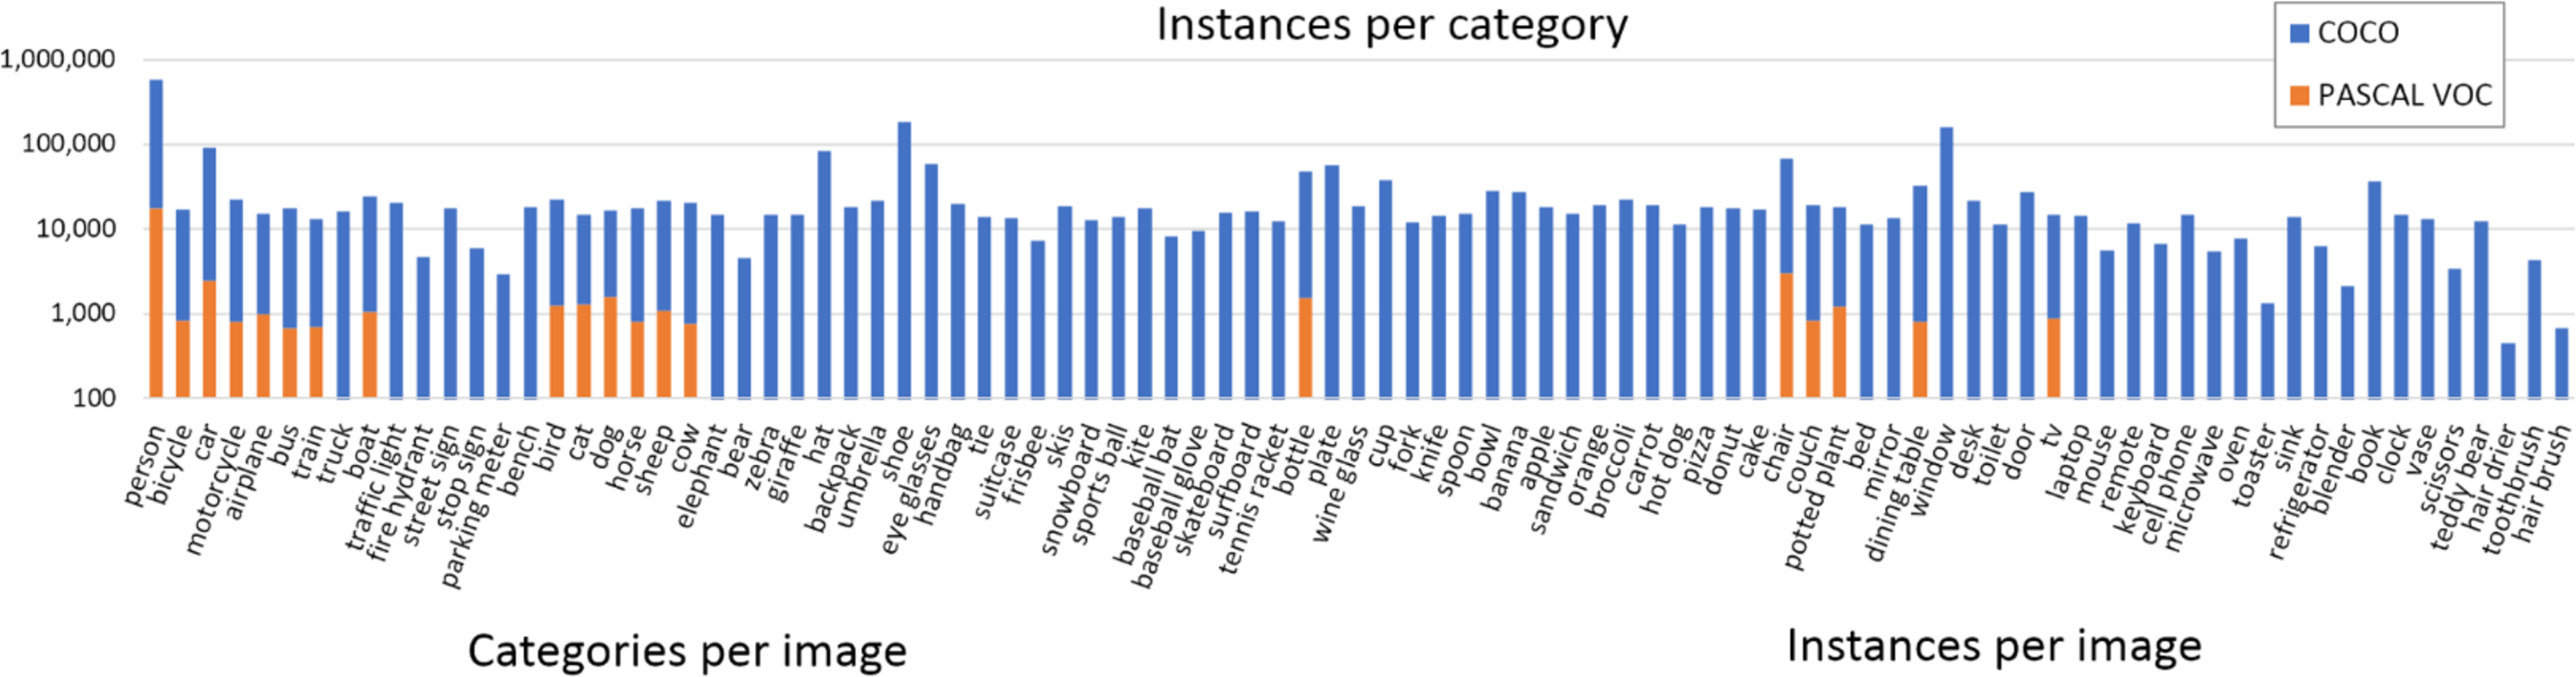
\includegraphics[width=1.0\textwidth]{Figs/Problem/mscoco_cats.pdf}
    \caption{Object categories and number of instances in each in the \gls{mscoco} dataset \cite{mscoco}.}
    \label{fig:cocoinstances}
\end{figure}


The image collection process was done using queries through Flickr inspired by the \gls{pascalvoc} method of collection. Having only a single categories as a query resulted in higher chances of iconic views, therefore multiple categories were used to collect images. Once collected and annotated the total number of images in the 2015 release was 328,000, split as 165,482 for training, 81,208 validation and 81,434 for testing.
\\\\
Apart from having a larger number of categories and there being a large number of instance per image (7.7), there are also other items that make this dataset more challenging. Firstly, the number of categories per image is larger than \gls{pascalvoc}, with 3.5 compared to 1.7. Additionally, the dataset is made up of much smaller images which are typically more difficult to detect. Roughly 65\% of object instances make up only 4-6\% of the total image size. This is in comparison to \gls{pascalvoc} at roughly 45\%.
\\\\
\gls{mscoco} uses 12 metrics to evaluate the performance of object detection, where 6 are variants of \gls{ap} and the remaining 6 variants of \gls{ar}. The \gls{ap} metric is calculated in the same manner as in \gls{pascalvoc}, however, the primary metric is also averaged over multiple \glspl{iou}. In \gls{pascalvoc} \gls{ap} is only calculated at \gls{iou}=0.5, however, in \gls{mscoco} \gls{ap} is average in the range of [0.50, 0.95] at intervals of 0.05. The \gls{mscoco} \gls{ap} is also evaluated on detections across ground truth image scales, as the number of small objects in the dataset is as mentioned relatively high. The scales covered is \gls{ap} for small objects that have a ground truth bounding-box are less than $32^2$ pixels, medium objects area between $32^2$ and $96^2$, and large objects with area above $96^2$. Apart from the primary metric and the three image scales, \gls{ap} is also calculated at two fixed \glspl{iou}. Firstly, at \gls{iou} 0.50 which results in the same metric as in \gls{pascalvoc} and at relatively strict \gls{iou} of 0.75. The \gls{ar} metric is also average across multiple \glspl{iou}, but also measure at a limitation of the maximum number of detections per image. This makes up three \gls{ar} metrics where maximum detections are 1, 10 and 100 per image. Finally the remaining three metrics evaluate the \gls{ar} across the same object scales mentioned earlier.